\chapter{Analyse et conception}

\section{Introduction}

Ce chapitre formalise le système : cas d'utilisation, scénarios dynamiques (dont le diagramme de séquence de l'assistant), diagramme de classes du domaine, schéma relationnel et architecture de déploiement. Les diagrammes UML suivent le guide ENSIASD pour la numérotation des figures \cite{uml}.

\section{Cas d'utilisation}

\subsection{Présentation du diagramme}

Le diagramme de cas d'utilisation (figure~\ref{fig:cu}) regroupe les fonctions autour de quatre paquets : commun, métier, administration et espace chauffeur. Tous les acteurs s'authentifient par JWT. L'administrateur et le responsable partagent la gestion des clients, chauffeurs, véhicules et missions, ainsi que le journal et l'assistant. Seul l'administrateur gère les utilisateurs et les rôles. Le chauffeur consulte ses missions, change le statut (démarrer / terminer) et met à jour son profil.

\begin{figure}[htbp]
\centering
\IfFileExists{figures/diagramme-cas-utilisation.png}{%
  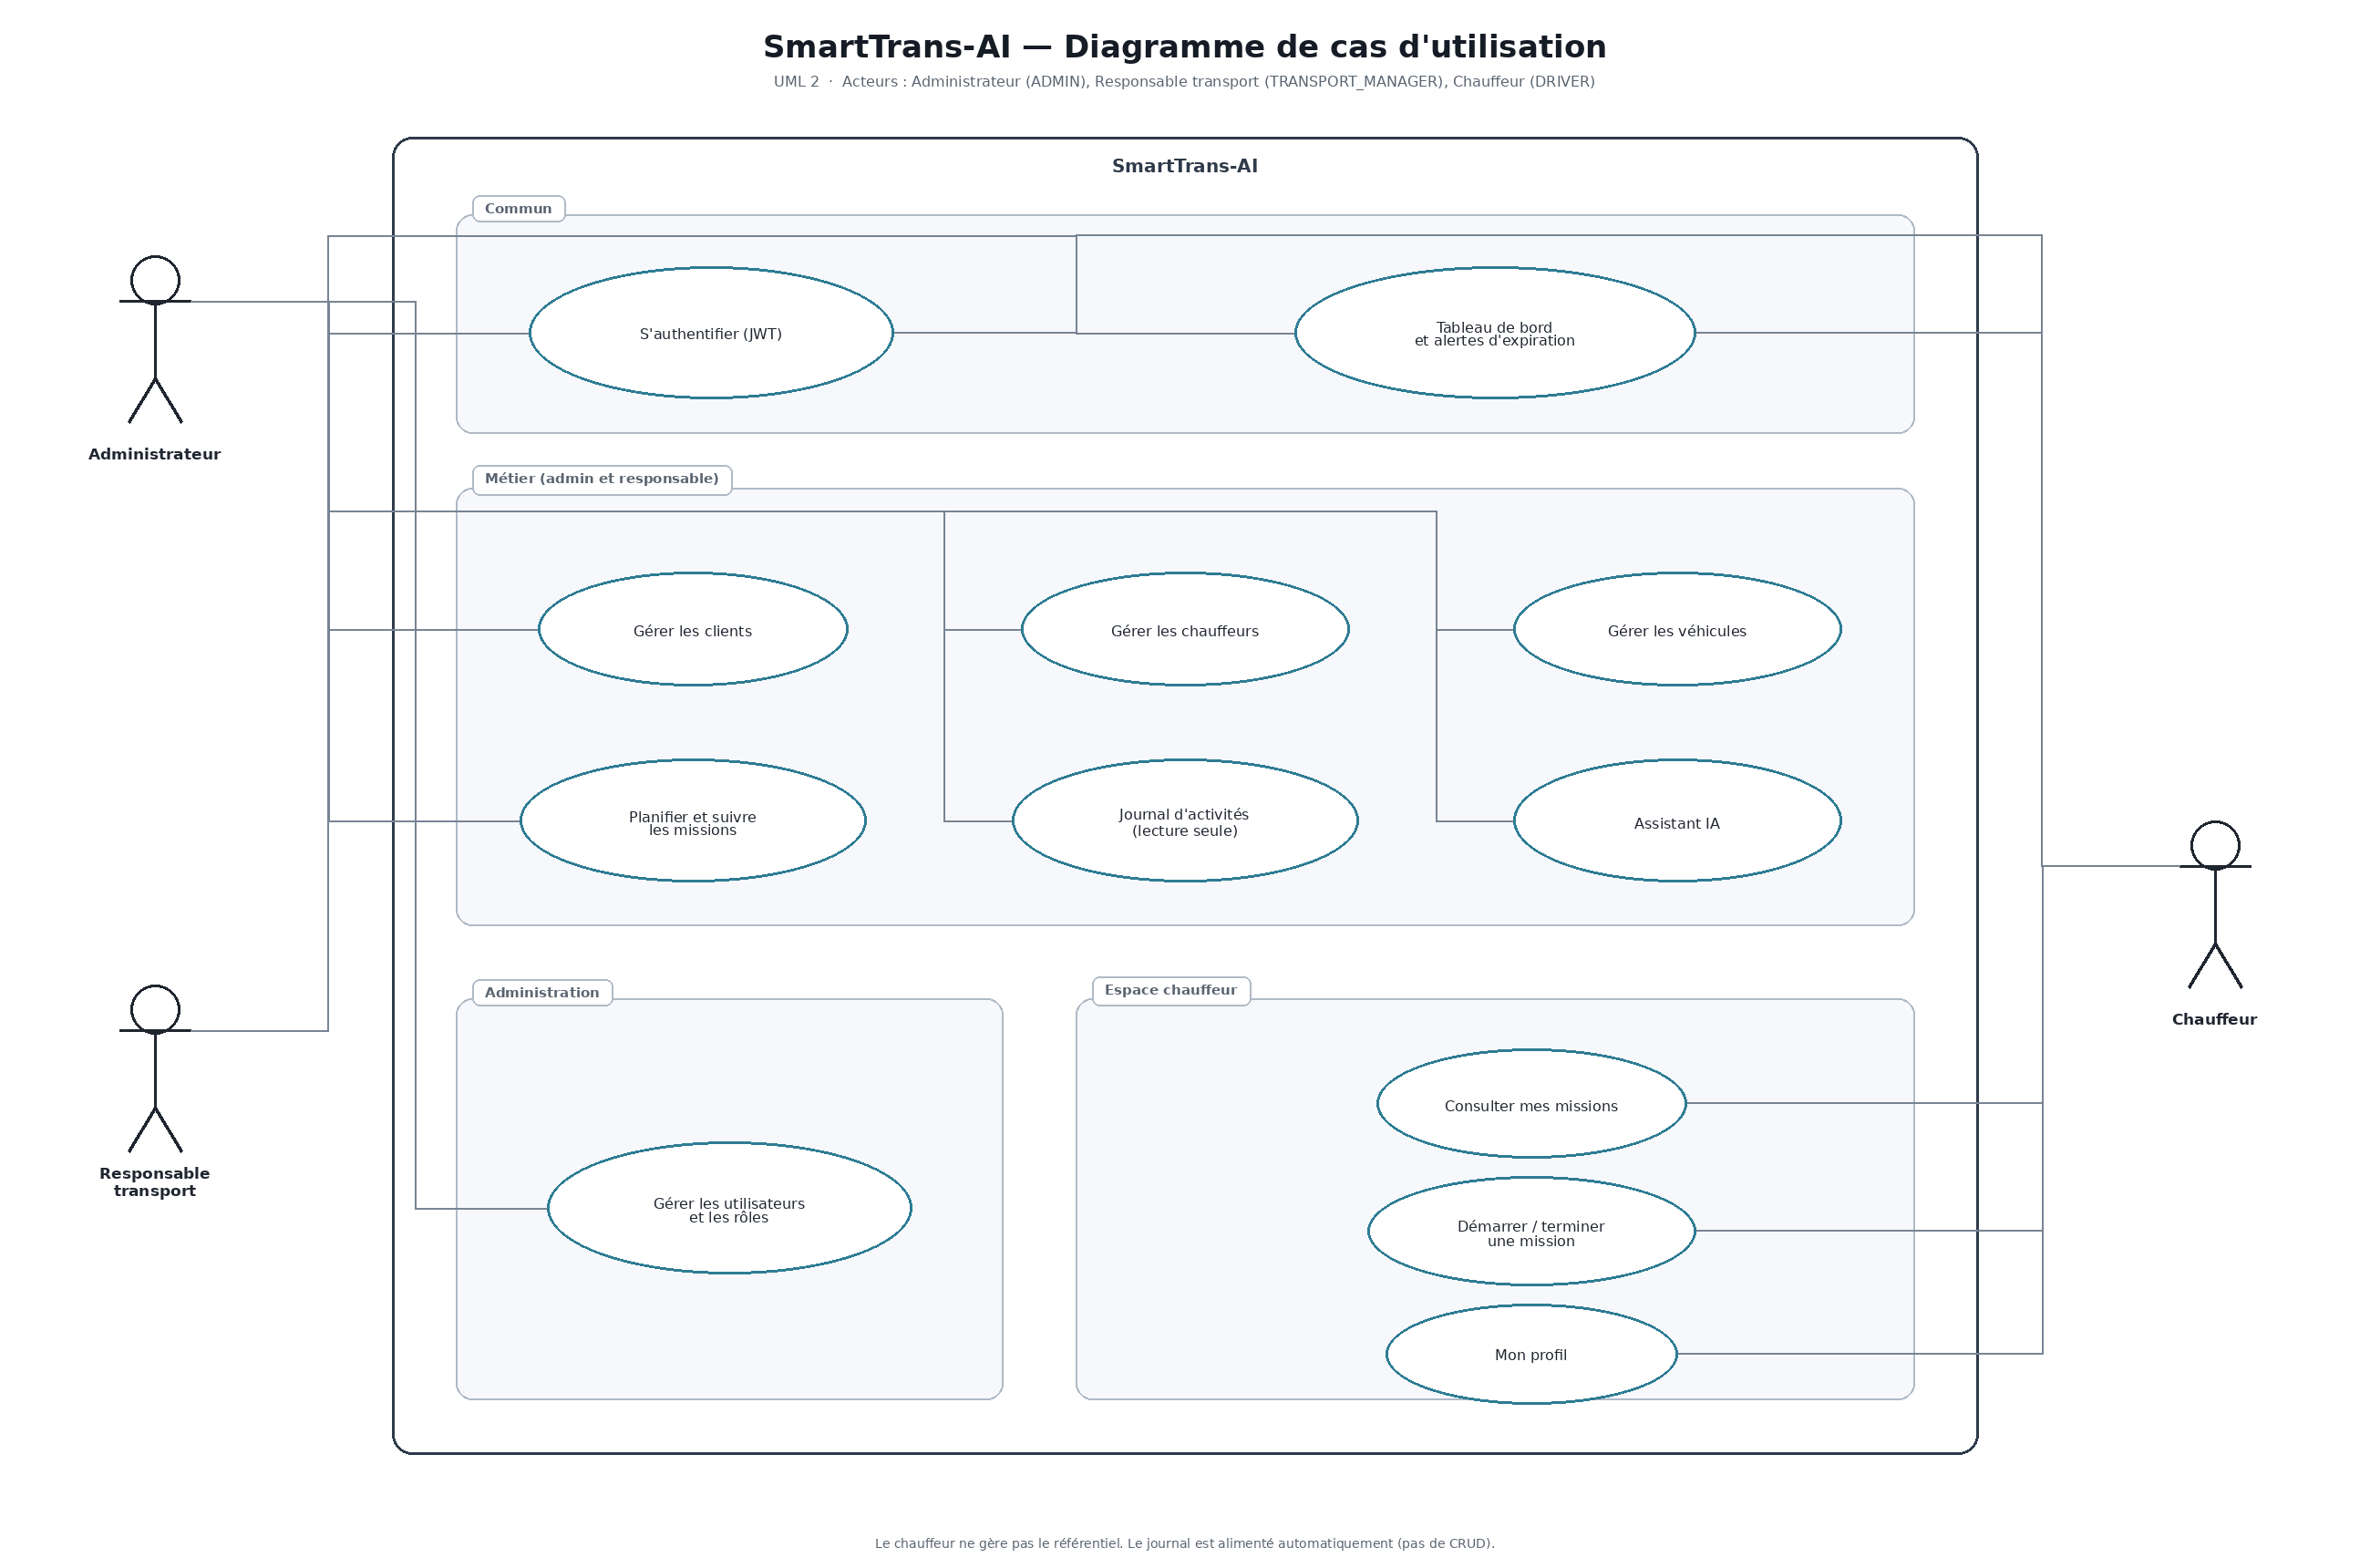
\includegraphics[width=\textwidth,keepaspectratio]{diagramme-cas-utilisation.png}%
}{%
  \FigPlaceholder{Générer \texttt{docs/soutenance/draw\_cas\_utilisation.py}\\vers \texttt{docs/rapport-stage/figures/diagramme-cas-utilisation.png}}%
}
\caption{Diagramme de cas d'utilisation de SmartTrans-AI}
\label{fig:cu}
\end{figure}

\subsection{Description des cas principaux}

L'authentification délivre un jeton utilisé sur les routes protégées. Le tableau de bord agrège des indicateurs (volumes de missions, graphiques, rappels d'expiration). La planification d'une mission associe un client obligatoire, un chauffeur et un véhicule optionnels, un trajet, une date et un statut (\texttt{PLANIFIED}, \texttt{IN\_PROGRESS}, \texttt{COMPLETED}, \texttt{CANCELLED}). Le journal est alimenté automatiquement (créations, mises à jour, suppressions, changements de statut, connexions) et n'offre pas de CRUD manuel. L'assistant répond à des questions du type effectifs de missions ou suggestions de chauffeur et de véhicule disponibles.

\subsection{Fiches de cas d'utilisation}

Les tableaux~\ref{tab:cu-auth} à~\ref{tab:cu-chauffeur} décrivent les cas les plus structurants, au format habituel (acteur, préconditions, enchaînement, exceptions).

\begin{table}[htbp]
\centering
\caption{Cas d'utilisation : s'authentifier}
\label{tab:cu-auth}
\begin{tabular}{|p{0.28\textwidth}|p{0.62\textwidth}|}
\hline
\TableHead
\tht{Identifiant} & \textcolor{white}{CU-AUTH} \\
\hline
Acteurs & Administrateur, responsable transport, chauffeur \\
\hline
Précondition & Compte existant, activé \\
\hline
Enchaînement & Saisie courriel et mot de passe ; vérification du hachage ; émission d'un JWT ; redirection vers le tableau de bord \\
\hline
Exceptions & Identifiants invalides, compte désactivé, origine CORS refusée \\
\hline
Postcondition & Le client conserve le jeton pour les appels suivants \\
\hline
\end{tabular}
\end{table}

\begin{table}[htbp]
\centering
\caption{Cas d'utilisation : planifier et suivre une mission}
\label{tab:cu-mission}
\begin{tabular}{|p{0.28\textwidth}|p{0.62\textwidth}|}
\hline
\TableHead
\tht{Identifiant} & \textcolor{white}{CU-MIS} \\
\hline
Acteurs & Administrateur, responsable transport (écriture) ; chauffeur (statut de ses missions) \\
\hline
Précondition & Client existant ; éventuellement chauffeur et véhicule disponibles \\
\hline
Enchaînement & Création (référence, trajet, date) ; affectation ; passage planifiée $\rightarrow$ en cours $\rightarrow$ terminée ; consultation des listes et filtres \\
\hline
Exceptions & Référence déjà utilisée ; chauffeur non affecté qui tente un changement de statut ; tentative d'annulation par le chauffeur \\
\hline
Postcondition & Mission persistée ; événement d'audit enregistré \\
\hline
\end{tabular}
\end{table}

\begin{table}[htbp]
\centering
\caption{Cas d'utilisation : espace chauffeur}
\label{tab:cu-chauffeur}
\begin{tabular}{|p{0.28\textwidth}|p{0.62\textwidth}|}
\hline
\TableHead
\tht{Identifiant} & \textcolor{white}{CU-DRV} \\
\hline
Acteur & Chauffeur \\
\hline
Précondition & Compte lié à une fiche chauffeur \\
\hline
Enchaînement & Consultation de mes missions ; démarrage ; clôture ; mise à jour du profil et de la disponibilité \\
\hline
Exceptions & Mission non affectée ; statut métier incompatible \\
\hline
\end{tabular}
\end{table}

\section{Scénarios dynamiques}

\subsection{Authentification}

Le navigateur envoie les identifiants à \texttt{POST /api/v1/auth/login} sans en-tête Bearer. L'API valide les informations, construit le jeton et renvoie le profil (rôles). Les appels suivants portent \texttt{Authorization: Bearer}. Un filtre ignore les routes d'authentification afin d'éviter un 403 sur le login.

\subsection{Cycle de vie d'une mission}

Le responsable crée la mission (statut planifiée). Le chauffeur authentifié appelle le changement de statut. Le serveur vérifie l'affectation et la transition autorisée, met à jour les horodatages \texttt{startedAt} / \texttt{completedAt}, et journalise l'action. L'annulation n'est pas exposée au profil chauffeur.

\subsection{Question à l'assistant}

L'administrateur ou le responsable transport saisit une question depuis l'interface. Le diagramme de séquence de la figure~\ref{fig:seq-assistant} détaille les échanges. Le navigateur envoie \texttt{POST /api/v1/assistant/ask} avec l'en-tête \texttt{Authorization: Bearer}. Le filtre JWT vérifie la signature et l'expiration du jeton. S'il est absent, invalide ou expiré, l'API répond \texttt{401} et l'utilisateur revient à l'écran de connexion, sans lecture des données.

Lorsque le jeton est valide, \texttt{AssistantService} interroge PostgreSQL et constitue un contexte ancré (missions, chauffeurs, véhicules, clients). Si une clé d'API est configurée, ce contexte est transmis à OpenAI (\texttt{POST /chat/completions}) et la réponse porte le mode \texttt{LLM}. Sinon, ou si l'appel échoue, le service compose lui-même une réponse courte, par exemple un effectif de missions (mode \texttt{GROUNDED}). Dans les deux cas, le client reçoit le texte, le mode et les citations, puis les affiche.

\begin{figure}[htbp]
\centering
\IfFileExists{figures/diagramme-sequence.png}{%
  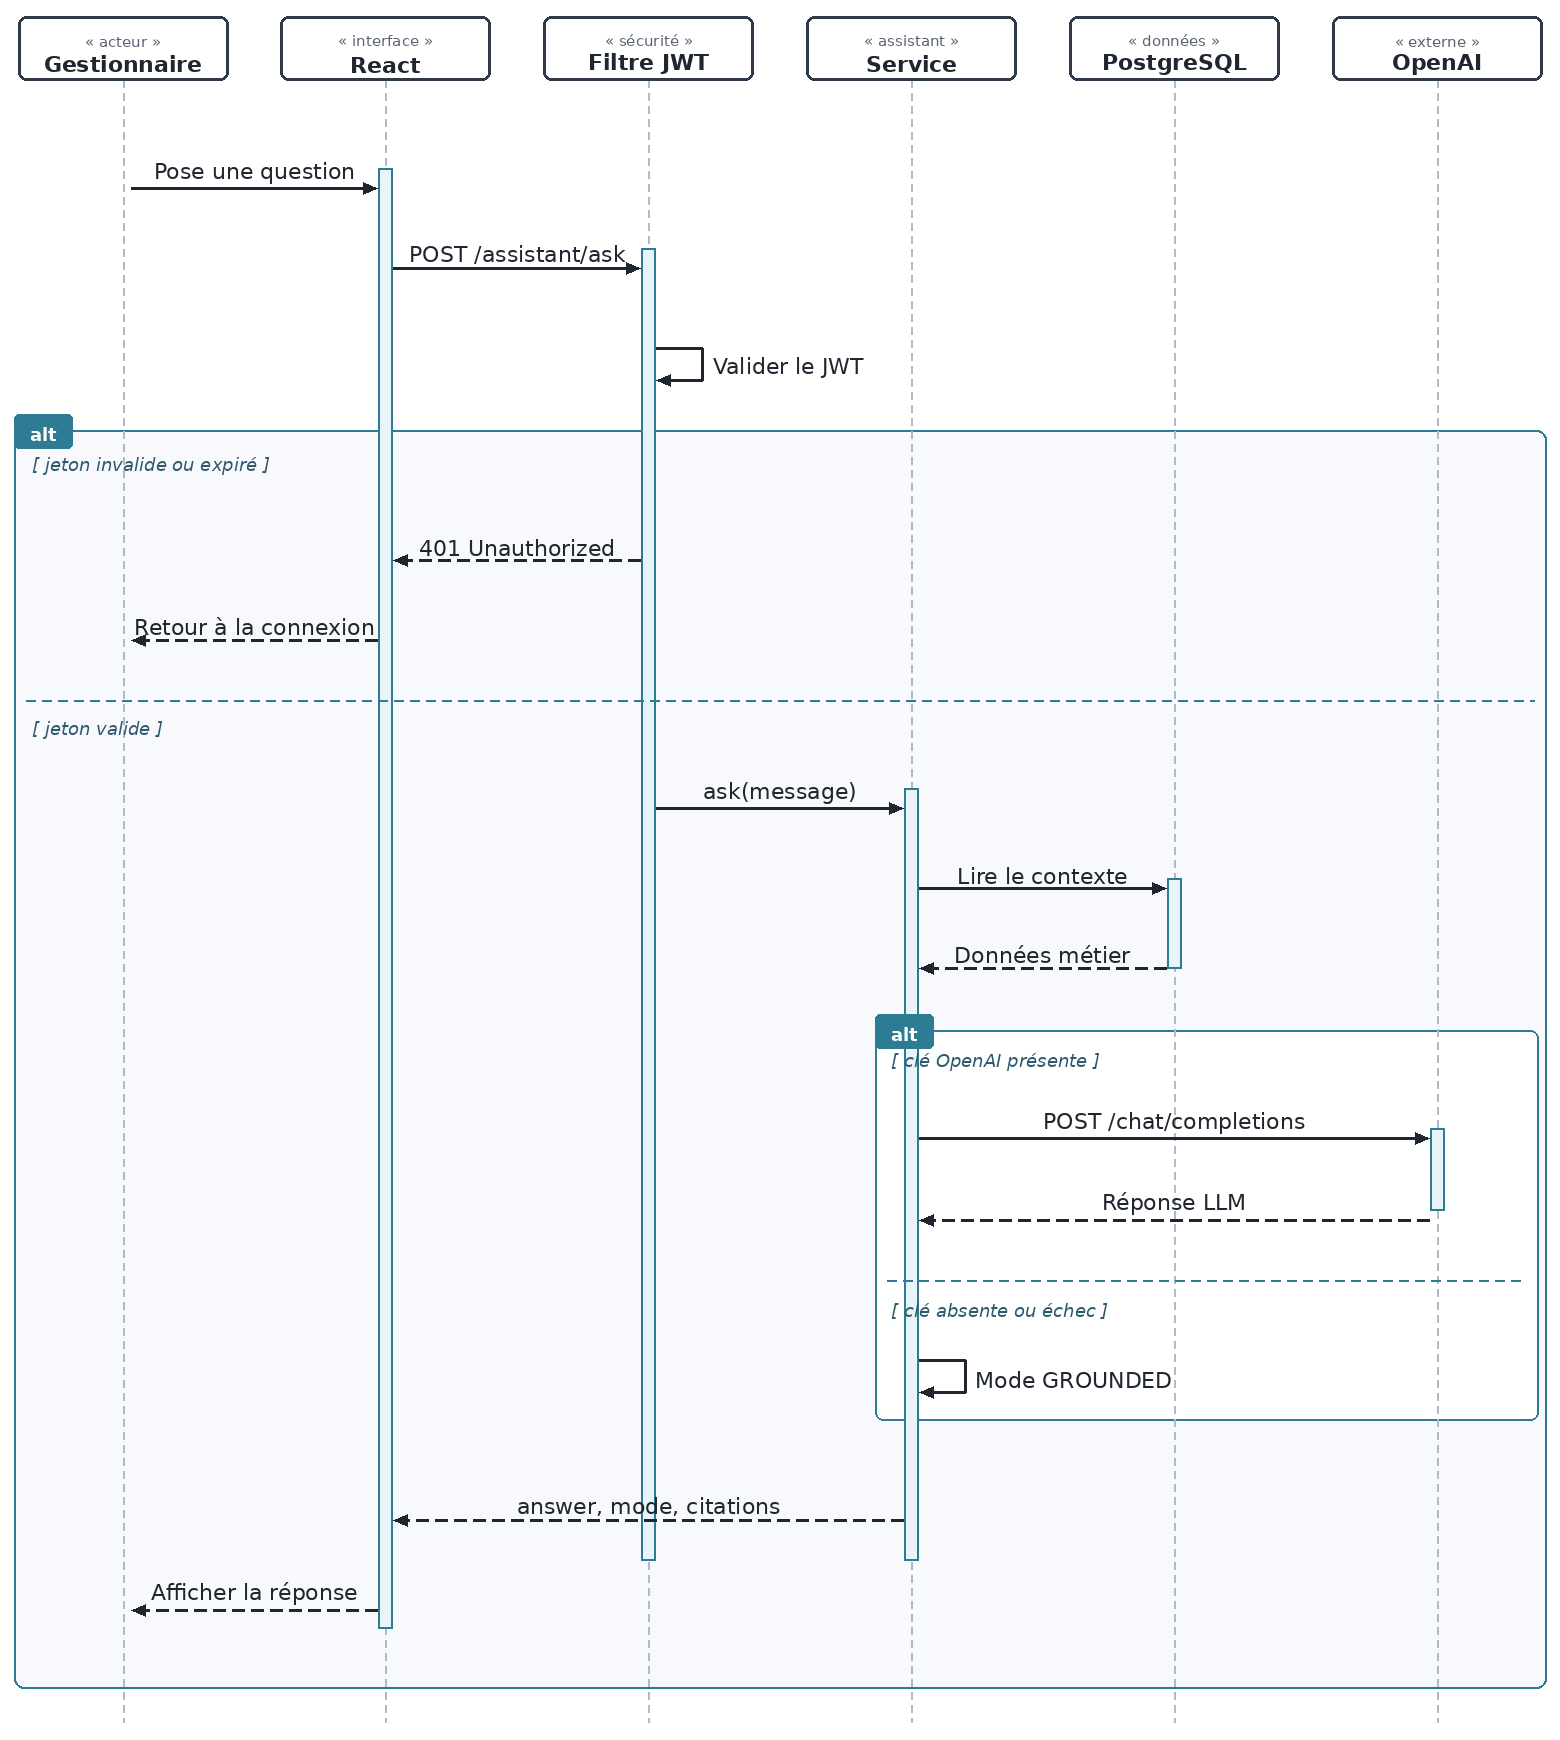
\includegraphics[width=\textwidth,keepaspectratio]{diagramme-sequence.png}%
}{%
  \FigPlaceholder{Générer \texttt{docs/soutenance/draw\_sequence\_assistant.py}\\vers \texttt{docs/rapport-stage/figures/diagramme-sequence.png}}%
}
\caption{Diagramme de séquence de la question à l'assistant IA}
\label{fig:seq-assistant}
\end{figure}

\clearpage
\section{Diagramme de classes}

\subsection{Entités du domaine}

\begin{figure}[htbp]
\centering
\IfFileExists{figures/diagramme-classes.png}{%
  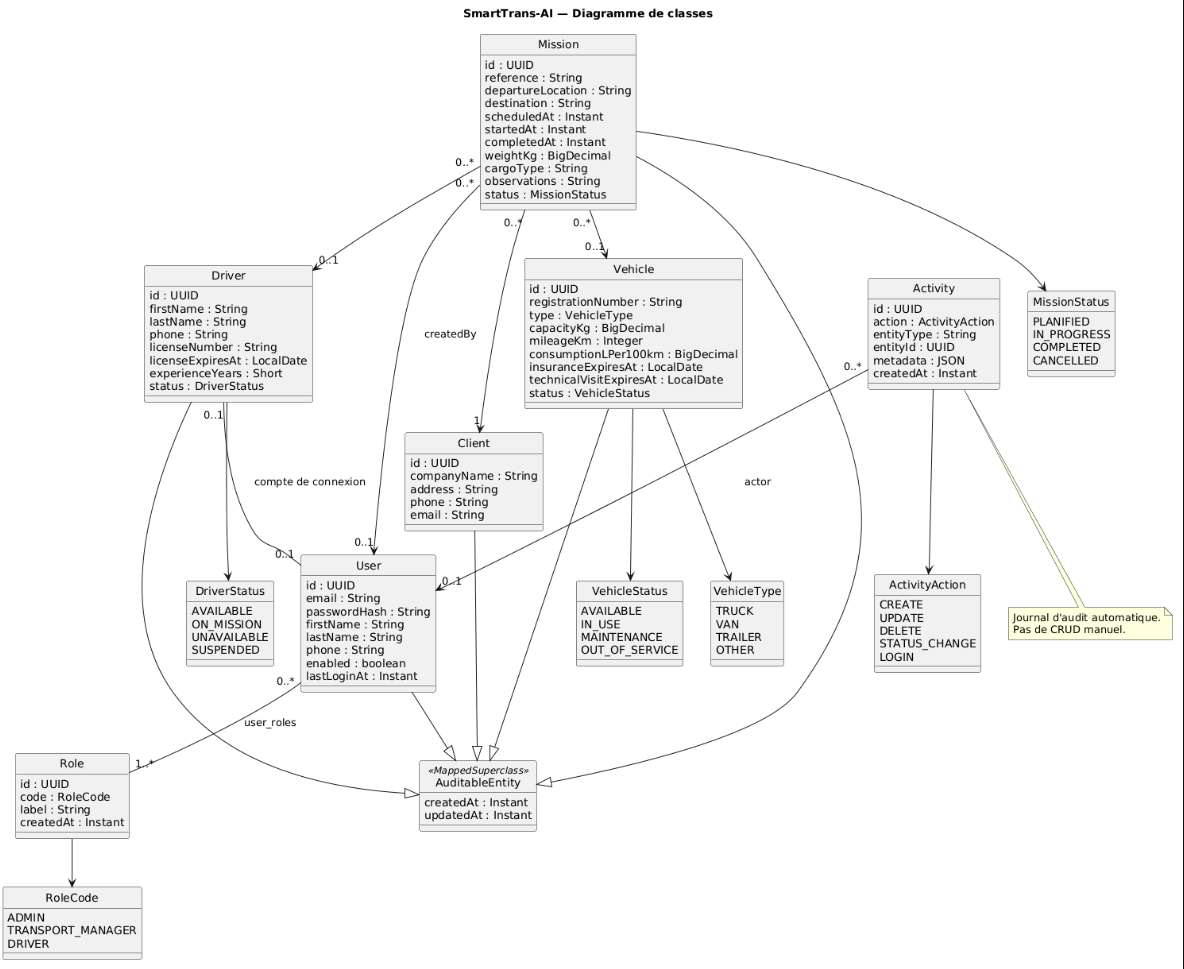
\includegraphics[width=0.92\textwidth]{diagramme-classes.png}%
}{%
  \FigPlaceholder{Exporter \texttt{docs/rapport/diagramme-classes.puml} en PNG\\vers \texttt{docs/rapport-stage/figures/diagramme-classes.png}}%
}
\caption{Diagramme de classes du domaine SmartTrans-AI}
\label{fig:classes}
\end{figure}

Le diagramme de la figure~\ref{fig:classes} représente le domaine persisté de SmartTrans-AI. Au centre, la classe \texttt{Mission} matérialise une course : référence, trajet, dates, tonnage et statut. Elle dépend d'un \texttt{Client} obligatoire et, le cas échéant, d'un \texttt{Driver} et d'un \texttt{Vehicle} ; l'association \texttt{createdBy} mémorise l'utilisateur qui a planifié la course. \texttt{User} et \texttt{Role} sont reliés par une association plusieurs-à-plusieurs (\texttt{user\_roles}), ce qui permet d'attribuer un ou plusieurs profils (administrateur, responsable transport, chauffeur). Un \texttt{Driver} peut être lié à au plus un compte \texttt{User}, afin que le chauffeur se connecte et suive uniquement ses missions. \texttt{Activity} constitue le journal d'audit : chaque action (création, mise à jour, suppression, changement de statut, connexion) pointe vers l'acteur. Les classes métier héritent de \texttt{AuditableEntity} (\texttt{createdAt}, \texttt{updatedAt}). Les énumérations \texttt{RoleCode}, \texttt{DriverStatus}, \texttt{VehicleStatus}, \texttt{VehicleType}, \texttt{MissionStatus} et \texttt{ActivityAction} limitent les valeurs autorisées. Les modules Document et Notification, hors périmètre livré, n'apparaissent pas sur ce diagramme.

\section{Modèle de données}

Les tables PostgreSQL correspondent aux classes : \texttt{users}, \texttt{roles}, \texttt{user\_roles}, \texttt{clients}, \texttt{drivers}, \texttt{vehicles}, \texttt{missions}, \texttt{activities}. Les identifiants sont des UUID. Le schéma est versionné par Flyway (validation au démarrage hors profil de test). Le tableau~\ref{tab:tables} synthétise les relations.

\begin{table}[htbp]
\centering
\caption{Principales relations du schéma}
\label{tab:tables}
\begin{tabular}{|p{0.28\textwidth}|p{0.28\textwidth}|p{0.34\textwidth}|}
\hline
\TableHead
\tht{Table} & \tht{Lien} & \tht{Cardinalité} \\
\hline
\texttt{user\_roles} & users -- roles & $n$--$n$ \\
\hline
\texttt{drivers.user\_id} & drivers -- users & $0..1$--$0..1$ \\
\hline
\texttt{missions.client\_id} & missions -- clients & $n$--$1$ \\
\hline
\texttt{missions.driver\_id} & missions -- drivers & $n$--$0..1$ \\
\hline
\texttt{missions.vehicle\_id} & missions -- vehicles & $n$--$0..1$ \\
\hline
\texttt{activities.actor\_user\_id} & activities -- users & $n$--$0..1$ \\
\hline
\end{tabular}
\end{table}

\section{Architecture logicielle}

L'interface React s'exécute dans le navigateur. En développement, le serveur Vite (port 5173) transmet les appels \texttt{/api} vers Spring Boot (port 8080). En production conteneurisée, un serveur HTTP (Nginx) sert les fichiers statiques et reverse-proxifie l'API. PostgreSQL stocke le métier. Le schéma~\ref{sch:arch} résume les flux.

\begin{schema}[htbp]
\centering
\fbox{%
\begin{minipage}{0.94\textwidth}
\centering\vspace{0.85cm}
\begin{tabular}{c@{\hspace{0.18cm}}c@{\hspace{0.18cm}}c@{\hspace{0.12cm}}c@{\hspace{0.12cm}}c@{\hspace{0.18cm}}c@{\hspace{0.18cm}}c@{\hspace{0.18cm}}c@{\hspace{0.18cm}}c}

\includegraphics[height=1.05cm]{logos/chrome.png} &
{\Large$\rightarrow$} &

\includegraphics[height=1.05cm]{logos/react.png} &
{\large/} &

\includegraphics[height=0.70cm]{logos/nginx.png} &
{\Large$\rightarrow$} &

\includegraphics[height=1.05cm]{logos/spring.png} &
{\Large$\rightarrow$} &

\includegraphics[height=1.05cm]{logos/postgresql.png} \\[0.28cm]
\small Navigateur && \small React && \small Nginx && \small Spring Boot && \small PostgreSQL
\end{tabular}
\vspace{0.85cm}
\end{minipage}%
}
\caption{Architecture logique de SmartTrans-AI}
\label{sch:arch}
\end{schema}

\section{Conclusion}

L'analyse produit un système à trois acteurs, un domaine centré sur la mission, et une architecture présentation / API / données. Le chapitre suivant décrit la traduction de cette conception en logiciel.
